\documentclass[11pt]{article}
\usepackage{amssymb}
\usepackage{amsmath}
\usepackage{graphicx}
\bibliographystyle{unsrt}
\textwidth=430pt
\textheight=640pt
\hoffset=-50pt
\voffset=-80pt
%opening
\title{Gravitational waves from colliding black holes}
\author{Chris Pedersen}

\begin{document}
\maketitle
\begin{abstract}
A complete understanding of the LIGO detectors' ability to accurately measure spin parameters is of key importance to understanding the astrophysics of binary black hole systems. Of particular significance is an ability to determine spin orientations as a means of distinguishing between binary formation models. In this work we overview the core physics of gravitational waves, relativistic precession in binary systems, the LIGO detectors, and the techniques involved in parameter estimation. We then examine the specific effects of precession on a gravitational waveform. The technique of 'matching' between waveforms is used as a computationally cheap way to explore degeneracies in the parameter space. A series of signals are then injected into simulated detector noise, and a full parameter estimation is performed on the data segments. Using the match results as a guide, we target these injections to areas in the parameter space where we expect to be particularly sensitive and insensitive to spin parameters. Inference for a full range of inclinations and phases is performed, and we identify areas where spin orientations are consistently incorrectly recovered. We then briefly examine the impact the upcoming VIRGO detector will have on spin estimation.
\end{abstract}
\tableofcontents
\newpage

\section{Introduction}
\subsection{A Brief History}
The first\cite{obs} and subsequent\cite{obs2} observations of gravitational waves (GWs) came around the centenary of Einstein's theoretical prediction of their existence\cite{eins1}\cite{eins2}. Einstein noticed that a solution to the linearised approximations of his field equations took the form of a wave equation\cite{gw1}, and that the source of these waves would be an asymmetric, massive, rotating system, such as a binary star system. As the amplitude of the waves was predicted to be so incredibly weak, with strain amplitudes on the order of $10^{-24}$, at the time there was no hope of ever actually detecting them, and Einstein even questioned whether they were physically real at all\cite{eins3}. Observations of the Hulse-Taylor pulsar (PSR 1913+16)\cite{hulse} showed that the energy loss of the binary agreed perfectly with the rate predicted by gravitational wave emission, providing indirect evidence of GWs and resulting in the award of the 1993 Nobel Prize in Physics, but it was not until the construction of the Laser-Interferometric Gravitational wave Observatory (LIGO) that direct detection of gravitational waves became possible - a truly remarkable feat of science and engineering involving the most precise measurements ever made by several orders of magnitude.

Now that the existence of gravitational waves has been confirmed and their detection is possible we enter a new era of astronomy, and it is difficult to overstate the wealth of science that is now attainable in the coming decades. Gravitational waves can be used to study astrophysical phenomena that cannot be observed using electromagnetic radiation, such as binary black hole (BBH) systems where two inspiralling black holes merge into one, as well as being used in conjunction with electromagnetic observations in 'multi-messenger' astronomy where events such as supernovae and gamma ray bursts are thought to release both gravitational and electromagnetic radiation which can be studied in conjunction with one another\cite{mm}\cite{mm2}. In addition GWs can be used to conduct the closest tests of general relativity (GR) to date\cite{gr1}\cite{gr2} as well as to further inform the ongoing development of quantum gravity models\cite{qgrav}. Currently the LIGO network consists of two detectors, one in Hanford WA (H1), one in Livingston LA (L1), however there are three detectors that will be added to the network in the coming years, with VIRGO (V1) in Italy due to come online by the end of 2017, and with LIGO India and KAGRA joining later. In addition to this, there are also proposals underway for a space-based gravitational wave observatory, the Laster Interferometric Space Antenna (LISA)\cite{lisa} which would be able to explore a different frequency-range and therefore study a range of different astrophysical objects to those observed using earth-based detectors.

This project focuses on studying the merging of a binary system, known as a compact binary coalesence (CBC). This term includes the merging of binary neutron star systems and neutron star-black hole systems, but in this work we focus on the merging of BBHs, where we do not consider the internal structure of the compact binary objects unlike in the case of systems involving neutron stars. We focus on parameter estimation of BBH mergers, with a specific emphasis on inferring the spin parameters of the component BHs in systems where the spins are misaligned, and how they can be determined though careful analysis of LIGO data.

The work is structured as follows; first we present an overview of gravitational wave theory and the LIGO detectors. We then discuss the process of parameter estimation and the mathematical and computational techniques that are used. Next we consider the case of systems with misaligned spins where relativistic precession is manifested, and consider the specific set of challenges this raises for signal analysis and parameter estimation. The astrophysical significance of studying precessing systems is also discussed. In chapter 2 we introduce the concept of 'matching' as a method for quantifying the degenerecy between different waveforms with minimal computational effort, and use these matches to identify the parts of the parameter space that would be most fruitful to explore. In chapter 3 we describe the process of software injections, where simulated signals are inserted into detector noise and then recovered using the inference methods introducted in the introduction. This gives a way of probing the detector response to a given signal. We present results from a range of software injections guided by the match findings, and attempt to analyse how effectively the current infrastructure is capable of inferring spin parameters on precessing BBHs. Finally we briefly consider the impact of the upcoming VIRGO detector on spin inference. The majority of the computational tasks involved in this work are performed in the PyCBC environment\cite{pycbc}, including the generation of waveforms, simulations of the detector response to gravitational waves, finding the matches between waveforms and running inference on data segments.

\subsection{Gravitational waves and their sources}
A complete analysis is available in Hartle\cite{hartle}, but here we briefly overview the fundamental theory of gravitational waves. In the general theory of relativity, gravity is a consequence of the curvature of a 4-dimensional spacetime as described by the Einstein equation (in natural units):
\begin{equation}
R_{\alpha\beta}-\frac{1}{2}g_{\alpha\beta}R=8\pi T_{\alpha\beta}
\end{equation}
where $R_{\alpha\beta}$ is the Riemannian curvature tensor, $g_{\alpha\beta}$ is the metric tensor, $R$ is the Ricci scalar and $T_{\alpha\beta}$ is the energy-momentum tensor. This equation is essentially ten non-linear partial differential equations, where we use the Einstein summation convention to sum over all indices, and where indices run from $0$ to $4$ and all tensors are symmetric. Intuitively, the LHS of this equation can be thought of as the local curvature of spacetime, and the RHS quantifies the energy and momentum density. In the weak-field regime, where the curvature of spacetime is low, the metric tensor can be approximated as
\begin{equation}
g_{\alpha\beta}(x)=\eta_{\alpha\beta}+h_{\alpha\beta}(x).
\end{equation}
where $\eta_{\alpha\beta}$ is the Minkowski metric and $|h_{\alpha\beta}| \ll 1$ for all components. This metric can be substituted into the Einstein equation, and expanding in $h_{\alpha\beta}$ in first order and using the Lorentz gauage, the Einstein equation becomes
\begin{equation}
\square h_{\alpha\beta}=0
\end{equation}
where $\square$ is the D'Alembertian operator, with the condition that
\begin{equation}
\partial_\beta h^\beta_\alpha-\frac{1}{2}\partial_\alpha h^\beta_\beta=0.
\end{equation}
The general solution to this equation is

\begin{equation}
h_{\alpha\beta}=
\begin{pmatrix}
0 & 0 & 0 & 0\\
0 & a_+ & a_\times & 0\\
0 & a_\times & -a_+ & 0\\
0 & 0 & 0 & 0\\
\end{pmatrix}
e^{i\omega(z-t)}
\end{equation}
for a wave with frequency $\omega$ propagating in the $z$ direction. Here the $a_+$ and $a_\times$ terms represent the amplitudes of the 'plus' and 'cross' polarisations respectively. As a gravitational wave passes through an observer, spacetime is distorted along the spatial directions orthogonal to the propagation direction of the wave according to these polarisation amplitudes. A visualisation of this is shown in Fig. 1. It is this stretching and squeezing of spacetime that the LIGO detectors were built to detect.

\begin{figure}[h]
	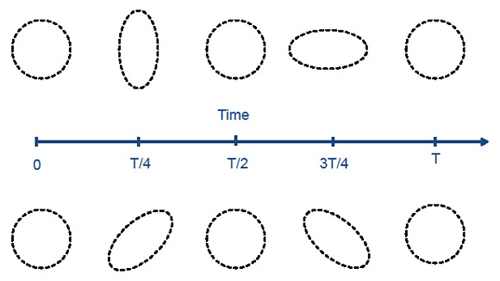
\includegraphics[scale=0.60]{fig1.jpg}
	\centering
	\caption{\cite{fig1}Plus and cross polarisations respectively of a gravitational wave propagating through the page, with scale greatly exagerrated.}
	\centering
\end{figure}

Now we consider the sources of these waves. Analysis in this area can rapidly become extremely complicated as the weak-field approximation is dropped and higher orders of perturbations are included\cite{blanch}, but the simplest case is still instructive.

\begin{figure}[h]
	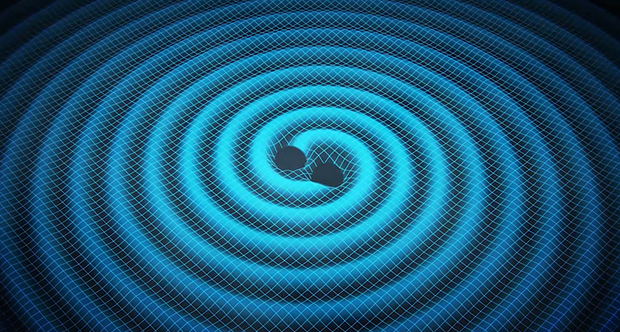
\includegraphics[scale=0.60]{fig2.jpg}
	\centering
	\caption{\cite{fig2}Impression of two inspiralling compact objects emitting gravitational waves}
	\centering
\end{figure}

Approximating that the field around the source is still weak, that the wavelength is long and that the observer is a large distance from the source, the spatial elements of the GW metric are
\begin{equation}
h_{ij}\approx\frac{2}{r}\ddot{I}^{ij}(t-r)
\end{equation}
where $I^{ij}$ is the second mass moment given by
\begin{equation}
I^{ij}(t)=\int d^3x\mu(t,\vec{x})x^jx^j
\end{equation}
where $\mu(t,\vec{x})$ is the mass density of the system. The energy loss of a binary system emitting gravitational waves is
\begin{equation}
L_{GW}=\frac{128}{5}M^2R^4\Omega^6,
\end{equation}
and as the binary loses energy, the separation between the compact objects decreases, increasing the orbital frequency. Given the connection between the mass distribution of the system in (7) and the GW amplitudes in (6), this gives rise to a 'chirp' effect seen in the signal of a CBC GW. This is shown in a Fig. 3. which is a simulated waveform of the merging of a BBH system.

\begin{figure}[h]
	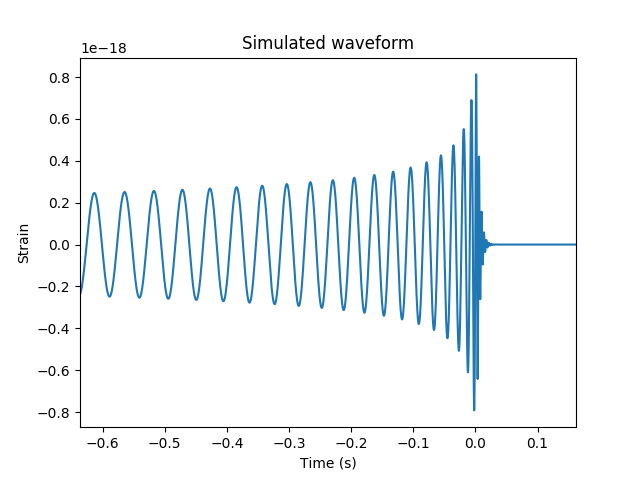
\includegraphics[scale=0.60]{fig3.png}
	\centering
	\caption{Simulated waveform of a BBH merger of two 35 solar mass black holes.}
	\centering
\end{figure}

The waveform can be split into three phases - the inspiral, the merger and the ringdown. The frequency, frequency evolution and amplitudes of each polarisation of the GW emitted from a merger will depend on the properties of the system itself, and as such there is information about the source contained in the specific morphology of a GW signal.

\subsection{LIGO}
\begin{figure}
	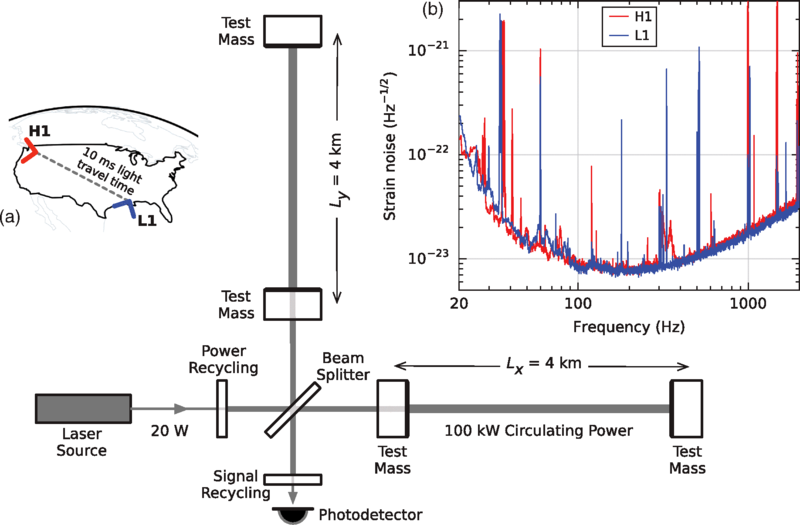
\includegraphics[scale=0.45]{fig4.png}
	\centering
	\caption{Simplified schematic of a LIGO detector\cite{advfig} showing noise curves and detector location}
	\centering
	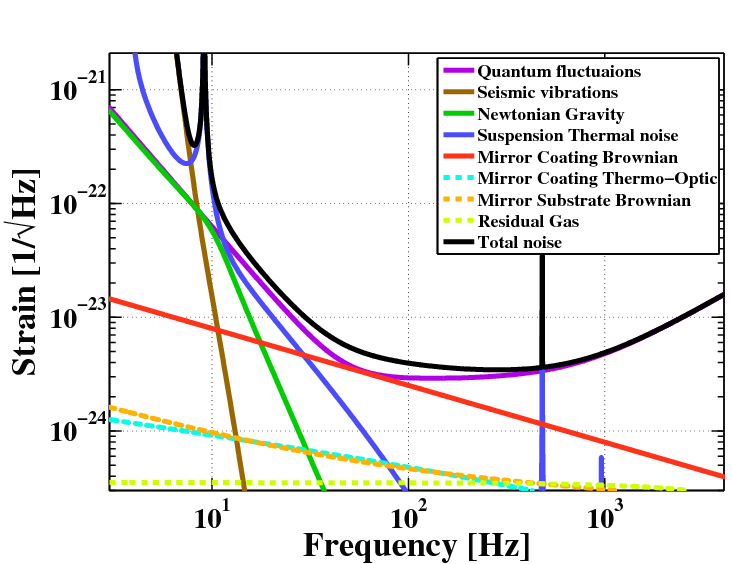
\includegraphics[scale=0.40]{fig5.png}
	\centering
	\caption{\cite{noisecurve}Noise 'budget for advanced LIGO detectors.}
	\centering
\end{figure}
The fundamental physical principle of the LIGO detectors is that they are laser interferometeres. Interferometers are devices that can measure extremely small changes in length to high accuracy using constructive and destructive interference, as shown in Fig. 4. Light leaves the laser beam, and is split down the two arms of the detector by the beam splitter. If the length of the two arms is equal, the optical path difference between the two light beams is zero, and the two beams constructively interfere after recombining at the beam splitter. However if there is any change in the length of one of the arms, the beams will no longer constructively interfere and the photodetector will register a change in intensity. As a gravitational wave passes through the detector, the relative length of the arms changes, and the GW signal is recorded by the photodiode. A large part of the scientific and engineering effort at LIGO involves techniques to minimise and account for noise in the system, and the recent advanced LIGO upgrade to the detectors increased the effective volume within which mergers can be detected by an order of magnitude\cite{noise}\cite{noise2}. Some of these techniques include suspending the mirrors from a series of pulleys and penduli, and applying real time corrections to the positions of the mirrors to compensate for external seismic noise. There is also considerable effort in managing the optics and lasers of the system in order to maximise the coherence of the laser beam and the intensity detected in the photodiode\cite{lasers}. The noise spectrum for advanced LIGO is shown in Fig. 5.\cite{noise3}, where the sharp noise peaks are specifically designed resonances that are removed from the strain data during signal processing. The strain data observed in the detector is a function of the different polarisation amplitudes
\begin{equation}
h(t)=F^{+}(\alpha,\delta,\psi)h_+(t)+F^{\times}(\alpha,\delta,\psi)h_\times(t),
\end{equation}
where $F^{+}(\alpha,\delta,\psi)$ and $F^{x}(\alpha,\delta,\psi)$ are the antenna beam patterns that describe how the detector responds to signals at different sky locations and polarisations\cite{beampat}. In first order, the polarisations are given by
\begin{equation}
h_+(t)=A_{GW}(t)(1+\cos^2(\iota)\cos(\phi(t)))
\end{equation}
\begin{equation}
h_\times(t)=-2A_{GW}(t)\cos(\iota)\sin(\phi(t))
\end{equation}
and binaries that are face on (with $\iota=0$) emit circularly polarised waves, and edge-on binaries emit linearly (either cross or plus) polarised GWs. On completion of the advanced LIGO upgrade in 2015 the network had a detection band of 10-7000 Hz, allowing BBH mergers to be detected up to a redshift of z=0.4\cite{lasers}. A variety of search algorithms continuously scan the data for a variety of signals\cite{search1}\cite{search2} using tailored triggers and template banks depending on the kind of search being conducted. Once a candidate signal is identified, the data around the event is then separated, and a more targeted and computationally intensive parameter estimation analysis is performed on it.

\subsection{Parameter estimation}
A signal is described by a total of 16 parameters\cite{props} - time and phase of coalesence $t_c$ and $\phi_c$, two parameters to describe sky location (right ascension, $\alpha$ and declination $\delta$), luminosity distance $D_L$, inclination angle $\iota$ describing the orientation of the binary's total angular momentum with respect to the line of sight, polarisation angle $\psi$, the masses $m_1$, $m_2$, six spin parameters to totally describe the spins on each of the two black holes $\vec{S}_1$, $\vec{S}_2$, and then two eccentricity parameters. In this work we ignore the eccentricity parameters and consider only circular orbits. The masses and spins of the component black holes are intrinsic parameters which determine the morphology of the waveform, and the remaining are extrinsic parameters. The maximum spin a black hole can have is $m^2$ in natural units, so the convention is to use a dimensionless spin magnitude $a=|\vec{S}|/m^2 \leq 1$. In the first order, the frequency evolution of the 'chirp' signal is approximated by a combination of the masses known as a the chirp mass
\begin{equation}
\mathcal{M}=\frac{(m_1m_2)^{3/5}}{(m_1+m_2)^{1/5}}\propto \bigg(f^{-11/3}\dot{f}\bigg)^{3/5}
\end{equation}
so the specific morphology of the waveform is in some sense determined by a combination of the total mass and the mass ratio. We also define the total mass $M=m_1+m_2$, and the mass ratio $q=m_2/m_1$ adopting the convention that $m1\geq m2$, so $0<q\leq1$.
Given that so many parameters, many of them extrinsic, describe only two sets of timeseries data (one from each detector), parameter estimation is a challenging task and the parameter space is both enormous and wrought with degenerecies. Two of the more thorougly researched degenerecies are those between total mass, distance and inclination, as all three parameters scale the amplitude of the signal and between mass and spin\cite{spindegen}, which is a degenerecy that arises out of post-Newtonian (PN) theory. 

The qualitative idea behind current methods of parameter estimation is that the GW signal is processed and extracted from the raw strain data, and then matched against an array of simulated waveforms to find which waveform most closely resembles the detected signal. The two technical challenges here are quantifying how well a template represents the observed signal, and how to efficiently sample the parameter space for new templates to test against the data. Within LIGO a standard method for quantifying the similarity between two signals $h_1(t)$ and $h_2(t)$ is given by the noise weighted inner product, also referred to as the 'match' between signals, and is defined as
\begin{equation}
\langle h_1(t) \vert h_2(t) \rangle=2\int_{0}^{\infty}\frac{\tilde{h_1^*}(f)\tilde{h_2}(f)+\tilde{h_1}(f)\tilde{h_2^*}(f)}{S_n(f)}df 
\end{equation}
where $\tilde{h}(f)$ is the Fourier transform of the signal $h(t)$, and $S_n(f)$ is the noise curve of the detector\cite{oldest_pe}. A variety of methods have been employed to sample the parameter space, including nested sampling\cite{pe2} and analysis using Gaussian wavelets\cite{props}, and in this work we use a framework of Bayesian inference and Markov-Chain Monte Carlo methods\cite{inj}\cite{pe}\cite{pe4}. This process results in a set of posterior distribution functions (PDFs) for each parameter. Using Bayes' Theorem, the posterior is given by
\begin{equation}
p(\vec{\theta})|d)=\frac{p(\vec{\theta})p(d|\vec{\theta})}{P(d)}
\end{equation}
where $\vec{\theta}$ is an $n$ dimensional vector in our parameter space of $n$ parameters\cite{pe2}. The first term in the numerator, $p(\vec{\theta})$ is known as the \textit{prior} distribution, and quantifies knowledge we already have about the system that should influence our estimation of its' parameters. In practice, in inference of BBHs, the priors are almost always uniform or isotropic distributions. The denominator, $P(d)$, is essentially a normalisation factor ensuring that the posterior distribution integrats to unity. The crucial term is the \textit{likelihood} for a given set of parameters given the data, which is determined by
\begin{equation}
p(d|\vec{\theta})\propto \exp\bigg(-\frac{1}{2}\sum_{k=1,2}\Big \langle h^M_k(\vec{\theta})-d_k \big\vert h^M_k(\vec{\theta})-d_k \Big \rangle\bigg)
\end{equation}
where the inner product is that defined in (13), $d_k$ is the observed strain in the detector, and $h_k^M(t;\vec{\theta})$ is the simulated detector response for a given set of parameters $\vec{\theta}$ given by (9).
Various methods of waveform generation (known as \textit{approximants}) have been attempted, with varying degrees of computational intensity. In general, Post-Newtonian expansions are used in the inspiral phase where the gravitational field is weak enough for approximations to be sufficient. During the merger and ringdown, full numerical relativity simulations are required as the curvature is sufficiently strong that Post-Newtonian approximations are no longer valid\cite{waveforms}\cite{imr}. These require significantly more computation time, and as such it is only in recent years that waveforms describing the full inspiral, merger and ringdown phases have become available.

--- some equation for SNR
--- overview of MCMCs that will be used for inference

\subsection{Precession and its astrophysical importance}
Considerable research has been done on studying non-spinning binaries and on non-precessing binaries where the spins are aligned or anti-aligned with the orbital angular momentum $\vec{\hat{L}}$\cite{pe3}, but it is only recently that a more complete study of the parameter space has begun\cite{sloos}\cite{pe_latest}. This is partly down to computational resources, as ignoring spin effects leads to a reduced parameter space and less computationally intensive waveforms. There are a unique set of challenges when considering binaries where the spins of the component black holes are not aligned $\vec{L}$, as due to relativistic effects, these binaries precess around the axis of total angular momentum $\vec{\hat{J}}$, giving a time dependence to the orbital plane of the binary\cite{precess1}\cite{precess2}.
\begin{figure}[h]
	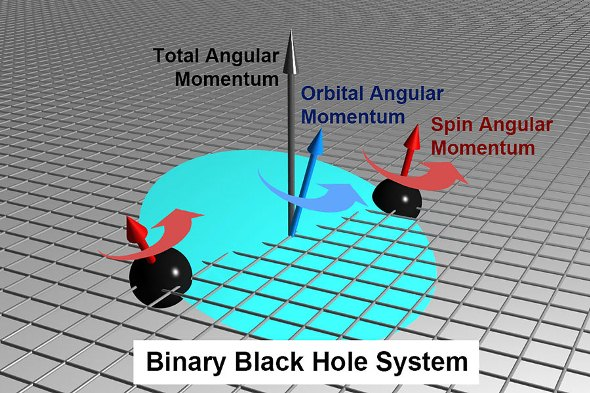
\includegraphics[scale=0.75]{fig6.jpg}
	\centering
	\caption{Illustration of a precessing binary system https://phys.org/news/2015-03-insights-black-hole-collisions.html}
	\centering
\end{figure}
This causes the signal in the detector to have an overall amplitude modulation as a function of time due to the change in orientation of the source, and therefore the change in direction of peak emission of GWs. This can be seen in Fig. 7, where we compare a very slightly precessing system with a maximally precessing one.
\begin{figure}[h]
	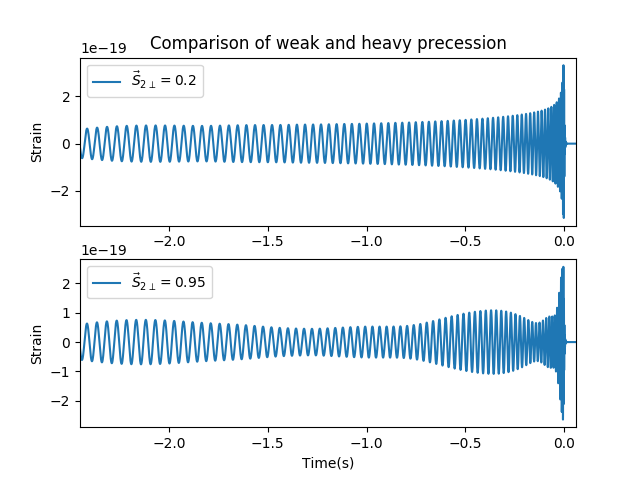
\includegraphics[scale=1]{fig7.png}
	\centering
	\caption{Waveforms for three BBH mergers with $m1=30$, $m2=10$ and with spins only in the $x$ direction on the heavier black hole. The inclination is such that the binary is viewed edge-on. LEGEND ON THIS FIGURE IS WRONG, FIX BEFORE SUBMIT}
	\centering
\end{figure}
Due to the computational intensity of dealing with both the generation of waveforms and inference process involving precessing systems, significant efforts have been made to reduce the size of the parameter space using the degenerecies between specific spin combinations to parametrise the spins of a binary. The most successful of these is the adoption of two spin parameters\cite{imr}\cite{chip} that describe the whole binary system, where we replace the six spin parameters with two:
\begin{equation}
\chi_{\text{eff}}=\bigg(\frac{\mathbf{S}_1}{m_1}+\frac{\mathbf{S}_2}{m_2}\bigg)\cdot\frac{\mathbf{\hat{L}}}{M}
\end{equation}
and
\begin{equation}
\chi_\text{p}=\frac{1}{B_1m^2_1}\text{max}(B_1S_{1\perp},B_2S_{2\perp})
\end{equation}
where $B1=2+3/(2q)$ and $B2=2+(3q)/2$. These parameters effectively quantify the amount of in-plane and out of plane spin of the total binary, removing large degenerate portions of the parameter space. As different spin configuations within these parameters are effectively degenerate, no loss of information occurs in this re-parametrisation. The recent adoption of this parametrisation in the generation of template waveform banks (the IMRPhenomPv2 waveforms which, we use in this work) has made exploring the precessing parameter space computationally viable, as it reduces the computation time by an order of magnitude. The results of these waveforms agree well when compared with waveforms generated using the full spin parameter space (known as the Spinning Effective One Body Numerical Relativity, or SEOBNR waveforms)\cite{spin}\cite{eob}, so the recent availability of a computationally efficient precessing waveform bank makes this an opportune time to conduct this research. Indeed the first full survey of an isotropic distribution of spins for a large number of simulations (200) has only very recently been published a matter of weeks ago\cite{pe_latest}.

The particular focus of this paper is on the challenges of inferring $\chi_p$ in precessing systems. This parameter is of particular importance due to its astrophysical implications, and as of yet there has been no comprehensive study into the effects of precession and it's amplitude modulation of the signal on the process of parameter estimation. The formation methods of compact binary systems of stellar mass black holes are currently unknown, and a variety of models have been proposed\cite{modal}. Of particular interest is whether the two black holes formed from a common accreting system, or whether the binary was formed by dynamical capture. The former model would imply that the spins on the black holes would generally tend to be aligned with one another and with the orbital angular momentum, however in the dynamical capture model we expect the spins to be more or less uniformly distributed. Given the large number of expected detections over the coming years, a thorough understanding of the detector's response to precessing waveforms and an accurate estimation of our ability to recover $\chi_p$ reliably will be crucial to answering these questions, and maximising the scientific yield from this remarkable technology.
\section{Intrinsic degeneracies}
\subsection{Precessing waveforms}
We first consider in more detail the effects of precession on a GW waveform. This is important as understanding how precessive waveforms behave is key to understanding how the detector will respond to these signals, and understanding the detector response is the fundamental idea of parameter estimation. A closer look at equation (16), which essentially quantifies the amount of precession in a given binary, shows that it takes values in the range $[0,1]$, with the maximum reached when the spin on the larger BH is fully in-plane. Even for a maximally precessing signal however, many possible configurations of polarisation and inclination are possible which will affect the way the amplitude of the signal is modulated. We show this in Fig. 8, where from this particular perspective the precessive effect appears largest in the case of the in-plane spin being $0.5$, instead of the maximally precessing system with $|\vec{S}|=0.98$. In this case, this is due to the fact that the inclination angle is defined with respect to the total angular momentum. In the case of precessing binaries, $\vec{L}$ and $\vec{J}$ are not aligned, so when we say we are viewing a binary 'edge-on', i.e. at $\iota=\pi/2$, the actual orbital plane of the system will not necessarily be edge-on. As a result, it is not always the case that precession affects are most noticeable in systems with the most precession, and a lot depends on the specific combination of source location and the polarisation and inclination angles for a specific event.
\begin{figure}[h]
	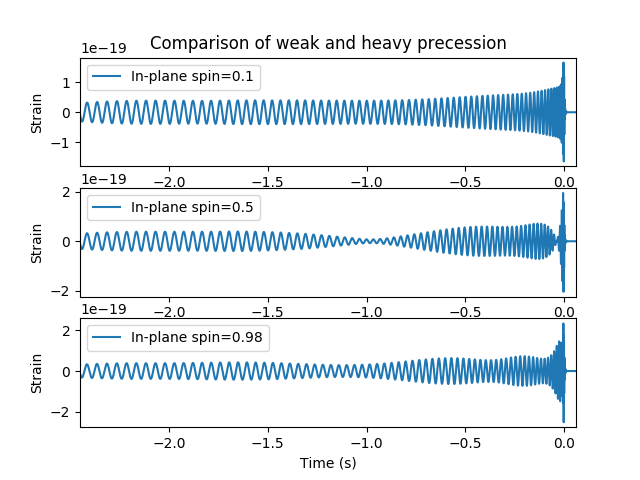
\includegraphics[scale=1]{fig8.png}
	\centering
	\caption{Waveforms for three BBH mergers with $m1=30$, $m2=10$ and with spins only in the $x$ direction on the heavier black hole. The inclination is such that the binary is viewed edge-on.}
	\centering
\end{figure}
The situation is further complicated by the fact that the phase, $\phi_c$ is an important degree of freedom in precessing binaries, as shown in Fig. 9. In non-precessing binaries, the phase is very much a trivial parameter which contains no interesting information about the system, however in precessing binaries the phase has a significant affect on the signal modulation. This opens up the possibility of many different degeneracies between binaries with different intrinsic parameters but a certain combination of phase and source location, and makes studying precessing waveforms more challenging. When considering precession it is also important to note that heavier total mass binaries have considerably shorter inspiral phases, and therefore fewer oscillation cycles within the detection frequency band. So while they will have a stronger signal, there is less opportunity for precessive effects to manifest.
\subsection{Matching and exploring the parameter space}
An extremely useful and computationally cheap way to identify some of these degeneracies is through the process of matching as defined in (13). In the \textit{PyCBC} framework, the match is maximised over extrinsic parameters such as distance and source location that only affect the amplitude of a signal, and so is a useful tool for examining the similarities in the morphologies of different waveforms. A match takes values in the range $[0,1]$, with identical waveforms having a match of 1. It is also important to note that the inclination parameter has a similar nature of that of the initial phase, in that in matches of non-precessing binaries it can be maximised over as it does not affect signal morphology, however once precession is added, waveforms at different inclinations no longer match, further adding to the complexity of the parameter space. In this section we intend to get some idea of the areas in which we expect the detector to be most sensitive to precession, and those in which precessing signals are intrinsically degenerate with non-precessing waveforms. This is done by incrementally changing waveform parameters and seeing how the match between the waveforms changes as a result. 
\begin{figure}[h]
	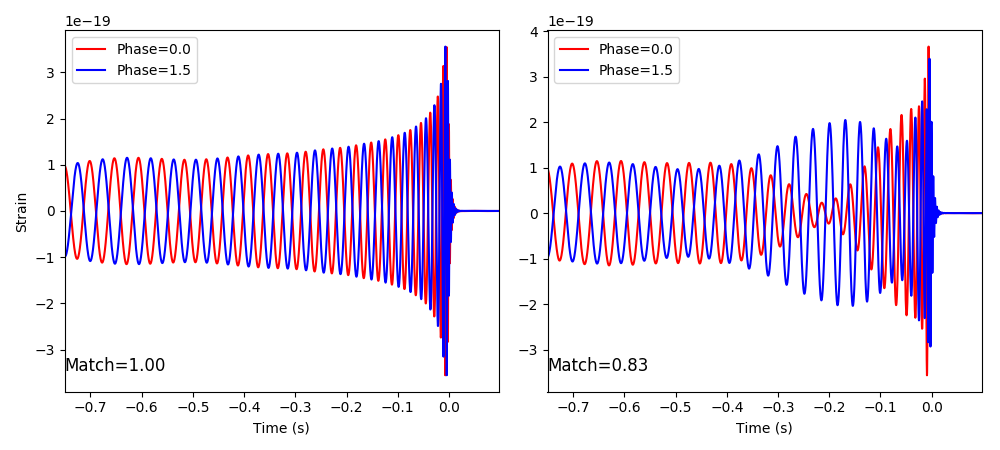
\includegraphics[scale=0.58]{fig9.png}
	\centering
	\caption{Affect of phase on non-precessing and precessing waveforms. Precession adds an extra degree of freedom in that the morphology of precessing waveforms is different for different phases.}
	\centering
\end{figure}
Fig. 10 shows how the matches between precessing and non-precessing waveforms change with inclination for four different mass ratios. The dark regions of the match is where the signals have significant mismatch, and the waveforms should be well distinguished, and hte light regions are where the waveforms are effectively degenerate. It is apparent that the degeneracy is far stronger for close to equal mass binaries, where only maximally precessing systems at edge-on inclinations will have noticeably different waveforms. Here we plot the 0.97 match contour as it is generally expected that the advanced LIGO detectors should be able to distinguish between waveforms with a match of 0.97. For all but the most extreme mass ratios, a combination of significant in-plane spin ($/geq0.6$) and/or strong inclination is necessary to have any significant deviation for systems with high precession. It is important to remember here that as we change the inclination, the overall strength of the signal will drop (with strongest at $\iota=0$), and the matching process does not account for this change in signal strength.

\begin{figure}[h]
	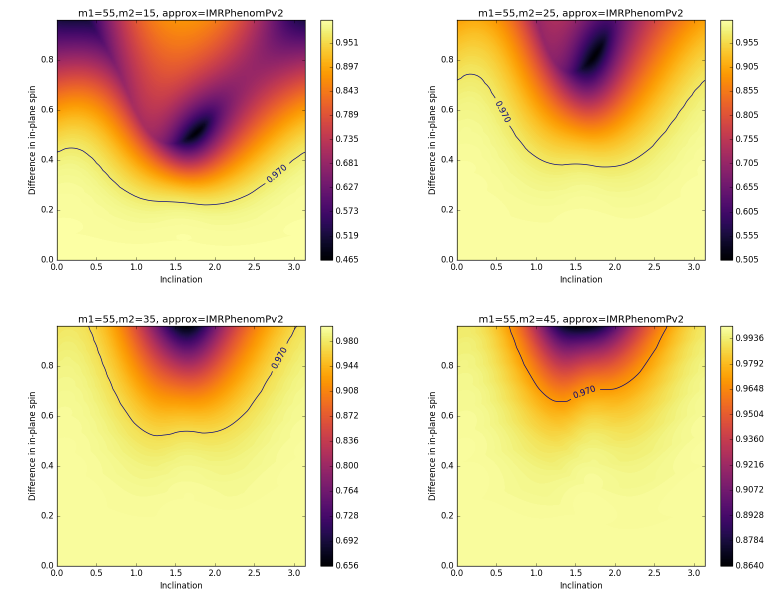
\includegraphics[scale=0.55]{fig10.png}
	\centering
	\caption{Matches between precessing and non-precessing waveforms for a range of inclinations and mass ratios.(make this more compact before submit)}
	\centering
\end{figure}

--Fig 11 will be spinDegen for 3 spins on 2nd BH

\begin{figure}[h]
	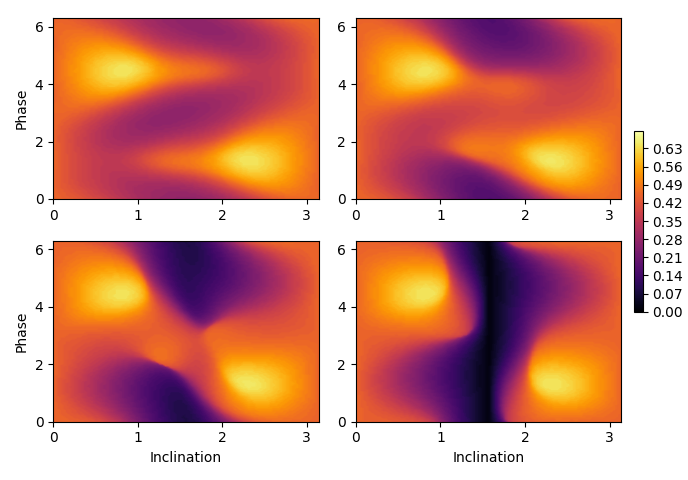
\includegraphics[scale=0.85]{fig12.png}
	\centering
	\caption{Match limit plots for a range of inclinations and phases for 4 polarisations.}
	\centering
\end{figure}

\section{Detector response simulations}
In this section we describe the process of inserting signals into simulated detector noise, and then perform a full parameter estimation.
\subsection{Signal extraction}
Data whitening - basically LOSC stuff, how we go from raw data to a signal - move this to intro?
\subsection{Inference pipeline}
A large number of software injections were going to be necessary to generate any interesting results due to the large size and complexity of the parameter space as revealed by the match results. So it was key that they could be performed efficiently and in an organised way. This required the construction of an inference pipeline which formed the bulk of the computational work of the project. This was ultimately one bash script that would create a new folder for each run, generate the injection file and run the inference MCMC.  It also saves the injected parameters as a python dictionary, plots all posteriors overlaid with injected parameters, plots the injected waveform, and the recovered (maximum posterior, or MAP waveform) and injected waveforms overlaid on the whitened detector strain data, and return matches between the MAP and injected waveforms. This meant that all the relevant analysis and data processing needed for each inference run was fully automated. A flow chart of this process is shown in Fig. 12.
This project work was also split between a number of different LIGO clusters, as well as work on several different local PCs, and so the pipeline along with all the relevant match and precession scripts were maintained as part of a GitHub repository which meant that the codes could be developed effectively and without conflict.
\begin{figure}[h]
	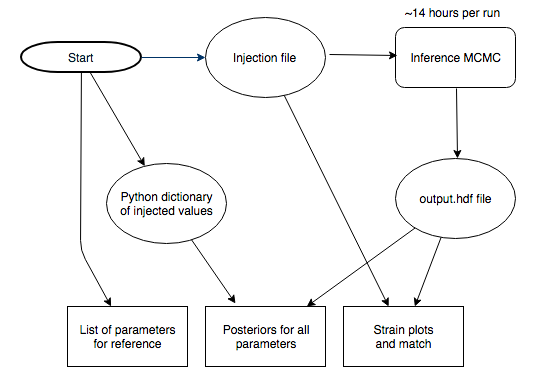
\includegraphics[scale=0.55]{fig13.png}
	\centering
	\caption{Flow chart of the inference pipeline. The ellipses represent data files that were generated during the pipeline and stored in case further analysis was necessary. The boxes at the bottom represent the final output of the pipeline.}
	\centering
\end{figure}
\subsection{Inference runs}
Posteriors and discussion of inference results. Great result that injected appears to match the signal better. Weakness in the inference pipeline? Perhaps its the case that match drops here due to the fact that precessive waveforms can often only really be significantly distinguished during the peaks of the merger phase. These are obviously susceptible to random noise fluctuations. Strong conclusion here.
\subsection{Impact of Virgo}
A look at how Virgo will influence PE, especially chi p estimation.
\section{Conclusions and implications}
Summary of results on PE and estimation of chi p, and a prospect on Virgo's impact.
\section{Reflective Statement}
I now need a therapist

Still to do:

1. SNR equation
2. MCMC description
3. Match plots for phase and inclination
4. Inference results - 2D posteriors
4. Inference results - strain plots
4. Inference results - Violin plots
5. Virgo results
6. Conclusions
7. Proper references of pics

\bibliography{draftbib.bib}
\end{document}
